\chapter{Diagrama de sequência}
\addcontentsline{toc}{chapter}{Diagrama de sequência}

Apresentação do diagrama de sequencia do projeto.

\begin{figure}[H]
    \label{figure_diagrama_sequencia}
    \centering
    \caption{Diagrama de sequência}
    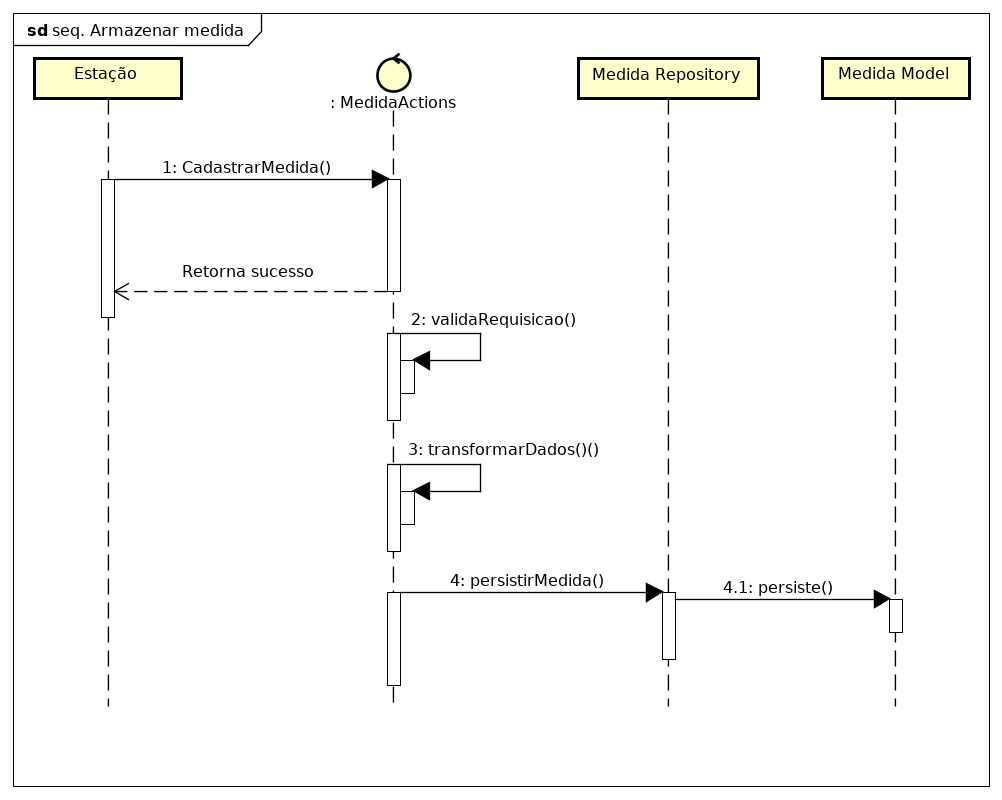
\includegraphics[scale=0.40]{diagrams/sequencia.png}
    \hfill
\end{figure}

Como descrito no diagrama de sequência representado na figura \ref{figure_diagrama_sequencia} a aplicação é composta por 3 principais camadas.

\section{Controlador}

Na camada de controle, os dados são recebidos e passam por uma básica validação através, porém não sofrem a interferência das regras de negócio.

Nessa camada, os dados são recebidos e retornados ao cliente, é uma interface de acesso a aplicação, geralmente, essa camada recebe objetos de requisições HTTP.

\section{Serviço de validação}

No serviço de validação, regras de negócio são aplicadas a medida para verificar se a mesma é valida para ser armazenada.

\section{Repositório}

Dentro da camada de repositório, são recebidos dados que, através de uma camada de infraestrutura são persistidos, retornando então, uma entidade.
